\documentclass{article}
\usepackage{iclr2027_conference,times}
\input{math_commands.tex}
\usepackage{graphicx}
\usepackage{booktabs}
\usepackage{microtype}
\usepackage{amsmath,amssymb}
\usepackage{xcolor}
\usepackage{enumitem}
\usepackage{hyperref}
\usepackage{url}

% Keep this empty for the double-blind ICLR submission.  Uncomment
% Enable the final-copy switch only after acceptance and author metadata review.
\title{When Governance Changes What Gets Counted: Measurement Validity for LLM Agent Evaluation}
\author{}

\newcommand{\high}{\textsc{high}}
\newcommand{\lastproposed}{\textsc{last-proposed}}
\newcommand{\pp}{\,\mathrm{pp}}

\begin{document}
\maketitle

\begin{abstract}
Runtime validators are intended to make language-model agents follow rules, but they can also change the population an evaluation scores. We study a conditional rate: among decisions whose response reports high water scarcity, how often does the agent increase demand? Because the agent writes this condition and the validator reads it, governance can change the rate by changing its denominator, not only the action.

The primary analysis compares validator-on and validator-off simulations across five seed-paired irrigation configurations. In the main irrigation configuration, no-validator runs have a $+45.73$ percentage-point higher share of high-scarcity reports and a $+23.02$ percentage-point higher conditional increase rate. Reweighting both arms to the same recorded world-state distribution leaves $-2.53$ percentage points at full coverage and $+0.21$ percentage points in the finest grouping, covering $43.4\%$ of governed and $36.4\%$ of no-validator decisions. Since governance changes world state, these comparisons are descriptive. Using an all-decision denominator changes one contrast from $+11.44$ percentage points to $+0.16$ percentage points and reverses its sign in another. As a secondary boundary check, nine Flood configurations span $-3.66\pp$ to $+6.24\pp$, whereas irrigation spans $+21.27\pp$ to $+47.53\pp$; this cross-testbed range check is not a mechanism-transfer test.

These results show a measurement-validity risk: a governed-agent score can change because its measured population changes. Report the condition share, an independent world-state record, and an all-decision rate beside any conditional score. Missing first responses prevent us from determining whether the agent would report the same condition in the same world; we make no deception claim.
\end{abstract}

\section{Introduction}

A runtime policy can change an evaluation score for two different reasons: it can change an action, and it can change which decisions enter the score. In an interactive agent system, the score is therefore not only a summary of actions; it is also a measurement procedure that defines the evaluated population. If a policy changes that population, a change in the score need not reflect a change in behavior alone. Agent benchmarks evaluate models in interactive environments, while agent frameworks expose action and feedback loops and runtime-enforcement systems add policies that inspect, reject, or retry responses \citep{liu2023agentbench,kapoor2024agents,yao2023react,shinn2023reflexion,wu2023autogen,yang2024sweagent,rebedea2023nemo,wang2026agentspec}.

The dependency becomes concrete when a response contains both an action and a condition about the current situation. Consider an irrigation agent that proposes increasing water demand while reporting high water scarcity. We call this field an \emph{agent-written condition}. If 80 of 100 decisions report high scarcity and 40 of those decisions increase demand, the conditional rate is 50\%. After governance, suppose that 40 decisions report high scarcity and 10 of those decisions increase demand. The rate is then 25\%. Both the numerator and denominator changed, so the two rates do not isolate an action change. The example does not require a deceptive agent; it follows from reusing one response field in two parts of the measurement pipeline.

Figure~\ref{fig:concept} summarizes this dataflow. The agent sends its proposed action to a validator, while the same agent-written condition enters the validator as a rule input and selects the records used in the conditional rate. An accepted action reaches the environment, and the final decision record enters the decision log before the measurement path counts records that satisfy the condition. The central object is therefore the shared condition that connects execution and scoring. The diagram abstracts the rule logic; it does not mean that a high-scarcity report alone is blocked. The conceptual diagram omits the retry and next-context paths for clarity; the Evaluation Setting and limitations describe their role, including the missing first response before a retry.

In a coupled environment, an accepted action can also change later state. A changed reservoir level, for example, enters the next decision's context and can affect future reports and actions. Governance can therefore alter the sequence of states from which later records are drawn. This setting is related to the statistical warning about conditioning on a variable affected by an intervention \citep{rosenbaum1984adjustment}. We use that warning to motivate a measurement audit, not to claim that the validator-on/off comparison identifies a causal effect.

Existing work has broadened agent evaluation beyond single-turn accuracy to interactive tasks and multidimensional assessment \citep{kapoor2024agents,liu2023agentbench}. Work on construct validity asks whether a benchmark measures the behavior it claims to measure \citep{bean2025construct}. However, these perspectives leave a specific runtime dependency underexamined: the system being evaluated can generate the condition that determines which of its own decisions enter the score. A conditional score can then change through record selection, while its action component is interpreted as if the denominator were fixed. Recording a parallel simulator state can help diagnose this dependency, but it does not make the state independent of governance when governance changes the environment before later decisions.

We study this problem primarily with validator-on and no-validator simulations in a coupled irrigation setting. The irrigation runs are paired by seed, and we compare (1) the share of decisions with the agent-written condition, (2) the conditional increase rate, (3) the increase rate over every decision, and (4) descriptive reweighting by simulator-recorded world state. We retain Flood only as a secondary numerical boundary check: it uses the same per-run-mean contrast, but its action space, feedback structure, prompts, and seed matching differ from irrigation. This check shows the scale of the contrast outside the primary setting; it does not test whether the irrigation mechanism transfers.

Our contributions are threefold:
\begin{enumerate}[leftmargin=1.3em,itemsep=0.1em,topsep=0.2em]
    \item We formulate a measurement-validity risk for runtime governance evaluations in which a condition authored in the response also selects the records used for scoring.
    \item We diagnose the risk with paired simulations, independent world-state records, and a cross-testbed check. In the frozen corpus, the large raw contrast is greatly reduced by descriptive alignment of recorded states, while all-decision rates can change its magnitude or direction; whether the agent would report the same condition in the same world remains unresolved.
    \item We give a minimal reporting protocol: show the condition share in both arms, preserve the independent world record, report an all-decision rate when the design permits it, and store the first response and validation message before a retry.
\end{enumerate}

All claims are descriptive and scoped to the evaluated governance loop. We do not claim that agents deceive, that the reweighting is a causal adjustment, or that the same magnitudes hold for every model or agent framework. The frozen corpus does not preserve the first response before a retry, so it cannot identify within-decision report revision; no result about that channel is assumed here.

The next section defines the paired evaluation and rule inputs. We then report the moving denominator, diagnose world-state composition, compare all-decision rates, and close with a reporting protocol and limitations.

\begin{figure*}[t]
    \centering
    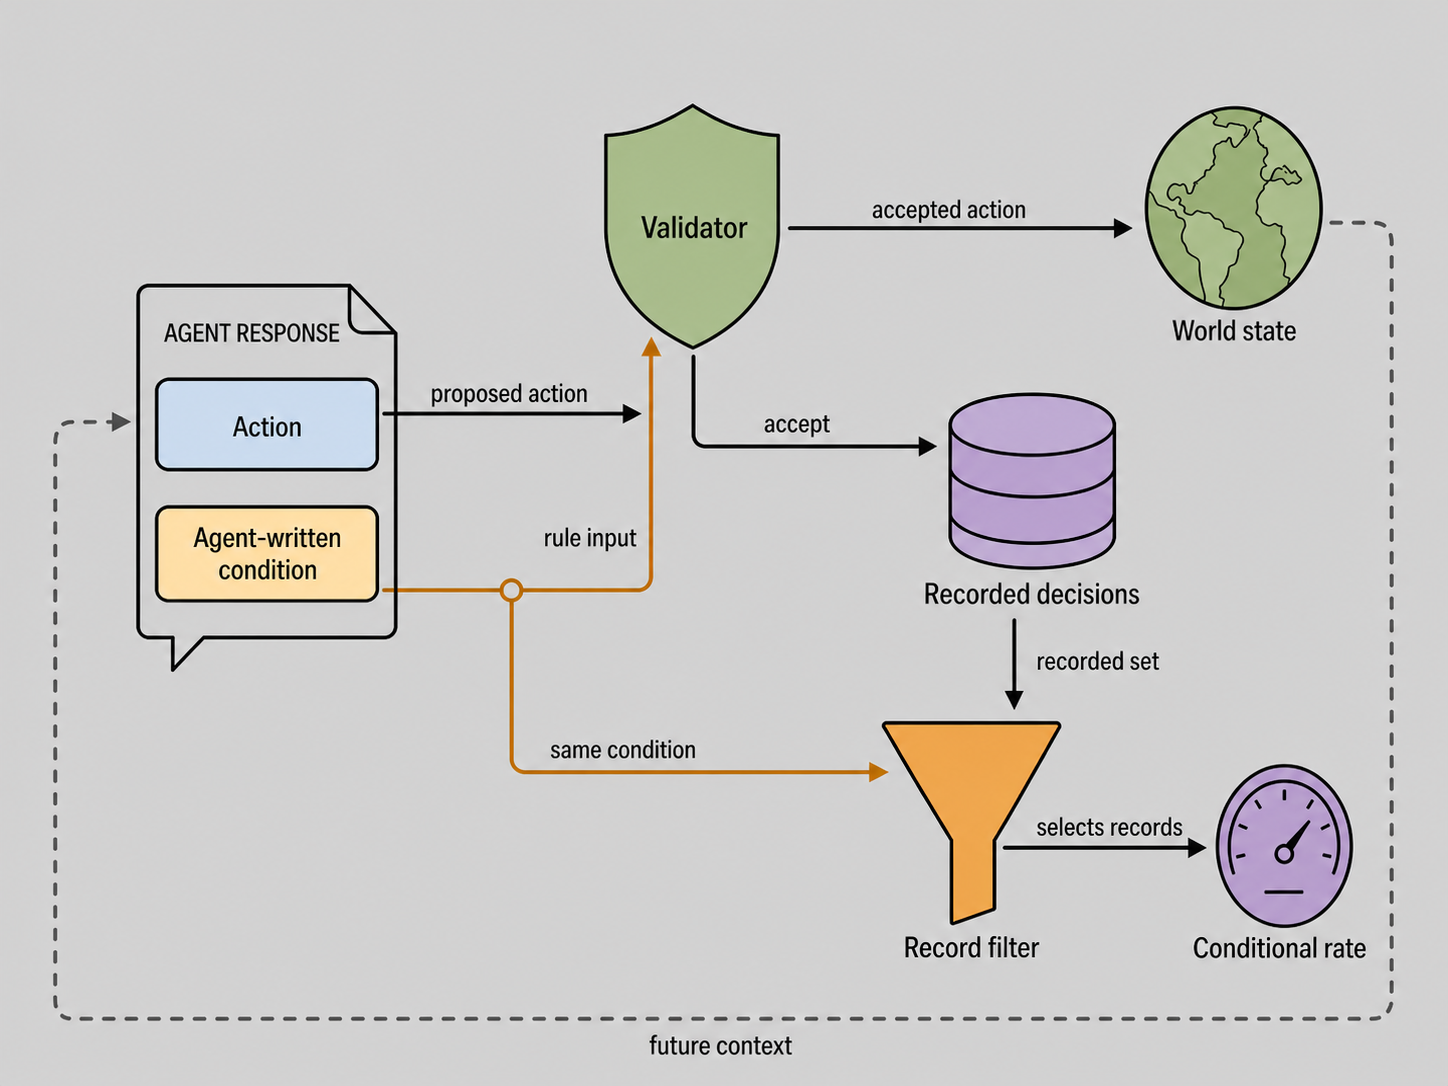
\includegraphics[width=0.98\textwidth]{../figures/active/figure1_concept.png}
    \caption{\textbf{How governance changes what gets counted.} The Agent response contains an action and an agent-written condition. The Validator reads the response before execution; an accepted action reaches the Environment, and the Validator's final record enters the Decision log. Colors encode roles rather than decoration: blue marks the agent response, orange marks runtime validation, green marks the environment, violet marks the measurement and record path, and amber marks the shared condition; black arrows and borders mark execution and record flow. For this paper, the displayed condition abstracts the primary scarcity report. The Counted records are logged decisions whose scarcity report satisfies that condition, and the conditional rate is the number of those decisions with an increase divided by the number of Counted records. The full validator rule also reads a separate coping-capacity report, and a high-scarcity report alone is not a blocking condition. Figure~\ref{fig:layers} gives the rule-layer decomposition. The observation-to-next-context loop and retry branch are omitted for clarity; the Evaluation Setting describes them, and the frozen corpus does not preserve the first response before a retry. This is a conceptual diagram, not a data figure.}
    \label{fig:concept}
\end{figure*}

\section{Evaluation Setting}
\label{sec:setting}

\subsection{Governance loop and rule inputs}

In each simulated decision, the agent returns an action and two conditions about its situation. A validator checks the proposal against agent-reported conditions and simulator-recorded state. If it finds an error-level violation, it returns a validation message and asks for a fresh response, up to three attempts. If the retry budget is exhausted, a domain default executes. The released audit record stores one row for each agent in each simulated year and uses the final proposed action, denoted \lastproposed, for the primary statistics. It does not store the first response before a retry.

The rule studied here is action-conditioned. It blocks an increase in demand only when the agent reports both high or very high water scarcity and high or very high coping capacity, where coping capacity is the agent's reported ability to adapt. This is the WAGF policy branch named \texttt{high\_threat\_high\_cope\_no\_increase}, not a conclusion inferred from the report. We study it for a structural reason: the same agent-authored fields are available to both the validator and the measurement denominator. High scarcity alone produces a warning rather than a block, preserving the agent's autonomy and the audit record. Thus, the block means that the increase proposal is ineligible under this testbed policy for that reported pair; it does not mean that high scarcity by itself justifies intervention. For the anchor irrigation cell, both conditions appear together in 25.46\% of governed decisions and 68.61\% of no-validator decisions, a $+43.15\pp$ contrast. The primary conditioning variable is the scarcity report. It is broader than the two-condition rule: it includes decisions satisfying both conditions and decisions with low coping capacity. We report this scarcity condition as the primary metric because it is the condition used by the frozen analysis; both quantities are agent-authored. A \emph{world state} is a condition recorded by the simulator rather than written by the agent, such as reservoir elevation or shortage tier.

The set of validator rules contains both types. Within that cell, 6,469 validator-on rejections are named by validator rules. Of these rejections, 59.4\% name at least one rule that reads a reported condition, and 40.6\% use only world-recorded conditions. The water-right cap is a separate eligibility check that also applies to increase proposals. Figure~\ref{fig:layers} locates the high-scarcity/high-coping increase rule among the self-report-conditioned blocks; the figure does not imply that all self-reported high scarcity is blocked. We therefore interpret the conditional rate only alongside this rule-layer decomposition.

\subsection{Paired simulations and quantities we compare}

Irrigation is the primary simulation setting. It contains 78 farm agents, 42 simulated years, and 3,276 decisions per run. A coupled reservoir makes an action in one year affect later world state. Five model configurations are evaluated in irrigation. Their validator-on and validator-off runs are paired by seed; most cells use five seeds and two irrigation cells use three. Flood contains nine additional model configurations and has no action-to-environment feedback. We use those artifacts as a quantitative but descriptive cross-testbed check: the high-threat-appraisal contrast is defined in both settings using the H/VH labels from the shared five-level appraisal instrument; irrigation stores it as \texttt{WSA\_LABEL} and Flood stores it as \texttt{TP\_LABEL}. The prompts, action ontology, feedback structure, and seed matching still differ. Across the two simulation settings, the corpus contains fourteen model configurations with publicly available weights spanning 3B to 27B.

For decision $i$ in seed $s$ and arm $a$ (validator-on or validator-off), let $R_{is}^a=1$ indicate an agent report of high or very high scarcity. Let $A_{is}^a=1$ indicate a demand increase in the \lastproposed action. With $N_s$ decisions in a seed, we report:
\begin{align}
    P_{\mathrm{high},s}^a &= \frac{1}{N_s}\sum_i R_{is}^a,\\
    r_{\mathrm{cond},s}^a &= \frac{\sum_i A_{is}^a R_{is}^a}{\sum_i R_{is}^a},\\
    r_{\mathrm{all},s}^a &= \frac{1}{N_s}\sum_i A_{is}^a.
\end{align}
The reported cell value is the mean of the per-seed values above. The contrast is always $\Delta=\text{off}-\text{on}$, so a positive value means that validators lowered the reported quantity. We report contrasts in percentage points (pp). The seed is the unit for inference. We use a two-sided one-sample $t$-test on the per-seed off-minus-on deltas; 95\% confidence intervals use the corresponding $t$ critical value with $n-1$ degrees of freedom. The reported $p$-values are cellwise and unadjusted for multiplicity, so the five-cell $p<0.05$ summary is descriptive rather than a familywise claim.

\section{The Denominator Moves}
\label{sec:denominator}

\subsection{Reported conditions and conditional rates}

The anchor irrigation cell makes the issue visible. With validators, high scarcity appears in 37.08\% of decisions; without validators it appears in 82.80\%. The share contrast is $+45.73\pp$ (95\% confidence interval (CI) $[+40.24,+51.21]$, paired $p<0.001$). Among decisions reporting high scarcity, the increase rate is 36.05\% with validators and 59.07\% without them, a contrast of $+23.02\pp$ (95\% CI $[+19.06,+26.98]$, $p=0.0001$). The rate and its denominator move together.

The pattern is not confined to the anchor model. All five irrigation configurations have positive share contrasts, ranging from $+21.27\pp$ to $+47.53\pp$; their cellwise, unadjusted $p$-values are all below 0.05. Table~\ref{tab:irrigation} reports these irrigation cells. It uses the same action reading and paired seed unit throughout. It makes a distinction that a single conformance score would hide: a lower conditional rate can coexist with a substantially different population of decisions satisfying the condition.

As a secondary boundary check, the nine Flood configurations span $-3.66\pp$ to $+6.24\pp$, and the two ranges do not overlap. Flood governance rejects 0--0.85\% of proposed actions, compared with 28--63\% in irrigation. We report this range in Table~\ref{tab:cross_testbed}; it is not a causal dose-response result or a test of mechanism transfer because the testbeds differ in field names, action ontology, feedback, and seed matching.

\begin{table}[t]
\caption{Irrigation condition shares and rates. \high{} is the share of decisions with a high or very high agent-reported scarcity condition. The conditional increase rate is computed only within \high{} decisions; the all-decision rate is in Figure~\ref{fig:consequence}. Values are per-seed means using \lastproposed. $\Delta$ is no-validator minus validator-on.}
\label{tab:irrigation}
\centering
\small
\setlength{\tabcolsep}{3.2pt}
\begin{tabular}{lrrrrrrr}
\toprule
Model & $n$ & \multicolumn{3}{c}{\high{} share} & \multicolumn{3}{c}{Conditional increase}\\
 & & on & off & $\Delta$ & on & off & $\Delta$\\
\midrule
gemma3:4b & 5 & 37.08 & 82.80 & +45.73 & 36.05 & 59.07 & +23.02\\
gemma3:12b & 3 & 5.49 & 26.76 & +21.27 & 5.45 & 16.89 & +11.44\\
gemma4:e2b & 5 & 18.26 & 65.79 & +47.53 & 12.71 & 31.65 & +18.94\\
gemma4:e4b & 5 & 45.27 & 88.65 & +43.38 & 23.67 & 41.08 & +17.41\\
ministral3:8b & 3 & 13.56 & 44.69 & +31.13 & 3.25 & 6.05 & +2.80\\
\bottomrule
\end{tabular}
\end{table}

\begin{table*}[t]
    \caption{\textbf{Secondary cross-testbed boundary check.} Values are ranges across model configurations; each configuration is computed from the mean of per-run means. $\Delta$ is no-validator minus validator-on. Irrigation stores the appraisal as \texttt{WSA\_LABEL} and Flood as \texttt{TP\_LABEL}; both use the high/very-high labels from the shared five-level instrument. This table is not part of the primary irrigation mechanism analysis: Flood is a descriptive range check rather than a paired comparison or a test of mechanism transfer. The Flood gemma3:4b configuration excludes one governed run with a divergent prompt, leaving four governed runs and five no-validator runs; including that run changes only this cell from $+0.35\pp$ to $-1.16\pp$.}
    \label{tab:cross_testbed}
    \centering
    \scriptsize
    \setlength{\tabcolsep}{4.5pt}
    \begin{tabular}{lrrrrr}
    \toprule
    Setting & Configurations & High-threat share on & High-threat share off & Contrast range & Mean $\Delta$ \\
    \midrule
    Irrigation & 5 & 5.49--45.27\% & 26.76--88.65\% & $+21.27$--$+47.53\pp$ & $+37.80\pp$ \\
    Flood & 9 & 2.55--43.48\% & 0.93--49.71\% & $-3.66$--$+6.24\pp$ & $+0.75\pp$ \\
    \bottomrule
    \end{tabular}
\end{table*}

\begin{figure*}[t]
    \centering
    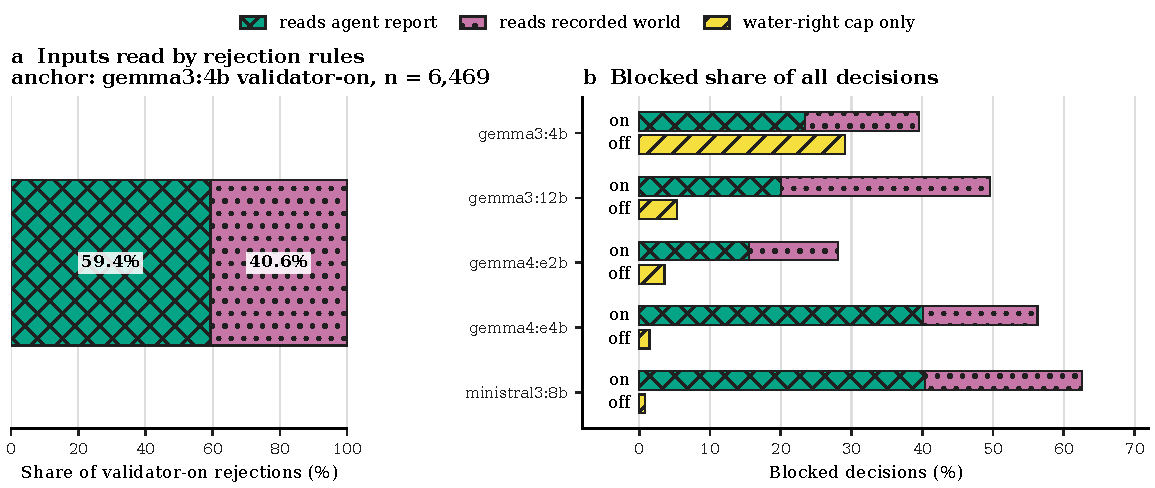
\includegraphics[width=0.98\textwidth]{../figures/active/fig1_rule_layers.pdf}
    \caption{\textbf{Rule-layer decomposition.} The anchor cell separates early eligibility failures from validator-named rejections. Among the 6,469 validator-on rejections, 59.4\% name a rule that reads an agent-reported condition and 40.6\% use only simulator-recorded conditions. The high-scarcity/high-coping increase rule belongs to the self-report-conditioned layer; high scarcity alone is a warning, not a block. The outer rows contain all decisions; the middle row recalculates percentages over only validator-on rejections and is not a third arm. Panel details and action counts follow the frozen evidence script.}
    \label{fig:layers}
\end{figure*}

\subsection{Why this is a measurement problem}

The conditional rate is not the fraction of all decisions that violate a rule. It is the rate of increase among decisions selected by an agent-authored condition. If validators alter the condition, the numerator and denominator no longer refer to a stable set of decisions. This does not tell us whether an agent changed its internal belief, nor does it show that a validator caused a particular action change. It tells us that the reported conditional score alone cannot distinguish those possibilities.

\section{World-State Composition as a Descriptive Mechanism}
\label{sec:world}

The coupled irrigation environment offers a direct diagnostic. An accepted increase affects the reservoir, and reservoir state enters later context. We use direct standardization: within each comparable recorded-world stratum, we compute each arm's high-scarcity share and then give both arms the same weights. The published pooled estimate uses the pooled counts from both arms in each comparable stratum. A stratum is comparable when it contains at least 40 records in each arm. Coverage is the fraction of all decisions in an arm that falls in the comparable strata. This asks how much of the raw difference remains after aligning the observed states; it does not recreate an identical world. These variables are outside the response being judged, but they are downstream of governance. The analysis is therefore a descriptive comparison of world-state composition, not a causal adjustment.

Using the anchor cell, the raw share contrast is $+45.73\pp$. Reweighting by shortage tier leaves a remaining difference of $-2.53\pp$ with 100\% coverage in both arms. A finer grouping of recorded states leaves $+0.21\pp$ with 43.4\% coverage in the governed arm and 36.4\% in the no-validator arm. These are pooled estimates after reweighting both arms to the same recorded-world distribution. The corresponding per-seed diagnostics are reported beside them in Table~\ref{tab:world} and in the supplement. For those diagnostics, each seed is reweighted using strata with at least eight records per arm. We report a paired interval only when at least three seeds retain comparable strata. The remaining difference is small relative to the raw contrast, but the analysis does not show that an agent would report the same condition in an identical world. Finer groupings trade coverage for resolution.

The environment itself diverges. The governed arm ends 106.57 ft higher on Lake Mead, with an average gap of 102.25 ft over the 42-year runs. The no-validator arm reaches the 895-ft floor in all five seeds, whereas the governed arm does not. At year 1, before actions can separate the worlds, the two arms match on nine pre-decision columns across 390 paired agent-years. The year-1 share contrast is $+3.33\pp$ (95\% CI $[-3.75,+10.42]$, $p=0.261$). The large later gap is therefore consistent with accumulated world-state composition.

The never-retried subset is a useful but limited sensitivity check. Its anchor contrast is $+53.46\pp$, larger than the all-decision contrast. The two arms are filtered differently, however: 36.2\% of governed decisions and 64.6\% of no-validator decisions are never retried. Because governance affects retries, this filtering can itself change the compared population. The comparison is therefore not evidence that selection is irrelevant.

\begin{figure*}[t]
    \centering
    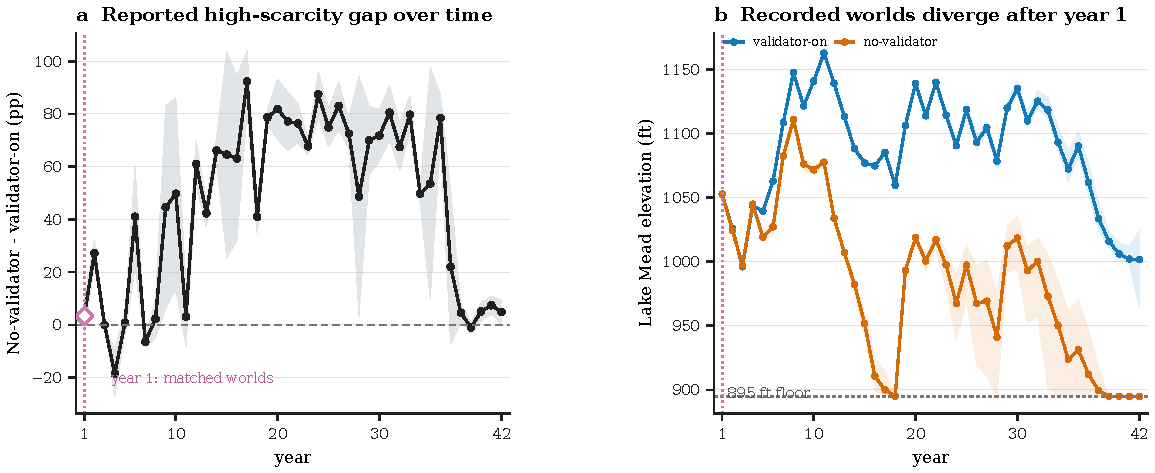
\includegraphics[width=0.98\textwidth]{../figures/active/fig2_mechanism.pdf}
    \caption{\textbf{Primary irrigation mechanism.} All three panels use the anchor irrigation cell. Panel (a) reports the yearly high-scarcity contrast, panel (b) shows the two recorded world-state trajectories, and panel (c) compares all decisions with the never-retried subset. Year 1 begins with matched pre-decision worlds; later reservoir divergence and unequal filtering make these panels descriptive rather than causal. The Flood boundary check is reported separately in Table~\ref{tab:cross_testbed} because its action ontology, feedback structure, field name, and seed matching differ from irrigation.}
    \label{fig:mechanism}
\end{figure*}

\begin{table}[t]
\caption{Selected world-state reweighting diagnostics for the anchor cell. The pooled difference is the no-validator minus validator-on share after reweighting both arms to the pooled recorded-world distribution. Coverage is reported as governed / no-validator. The per-seed diagnostic is a separate estimate with a paired 95\% interval.}
\label{tab:world}
\centering
\scriptsize
\begin{tabular}{lrrr}
\toprule
Stratification & Coverage (on/off) & Pooled difference ($\pp$) & Per-seed (95\% CI)\\
\midrule
Shortage tier & 100.0/100.0\% & -2.53 & -3.12 [-5.56,-0.68]\\
Finest reported rung & 43.4/36.4\% & +0.21 & -0.87 [-4.94,+3.19]\\
\bottomrule
\end{tabular}
\end{table}

\section{Different Denominators Answer Different Questions}
\label{sec:estimands}

The conditional rate asks: among decisions whose response reports high scarcity, how often is the action an increase? The all-decision rate asks: across every decision, how often is the action an increase? Neither is automatically the corrected answer. They answer different questions.

The contrast changes in every irrigation cell when the denominator includes every decision. On the anchor cell, it changes from $+23.02\pp$ conditionally to $+21.62\pp$ over all decisions. On gemma3:12b, it changes from $+11.44\pp$ to $+0.16\pp$ (95\% CI $[-13.92,+14.25]$, $p=0.965$). On ministral3:8b, the conditional contrast is $+2.80\pp$ while the all-decision contrast is $-22.17\pp$. These contrasts use \lastproposed{} actions. If we instead count the action that executed after a rejection, the gemma3:12b all-decision contrast becomes $+27.82\pp$. The action reading is therefore part of the quantity being compared.

\begin{figure*}[t]
    \centering
    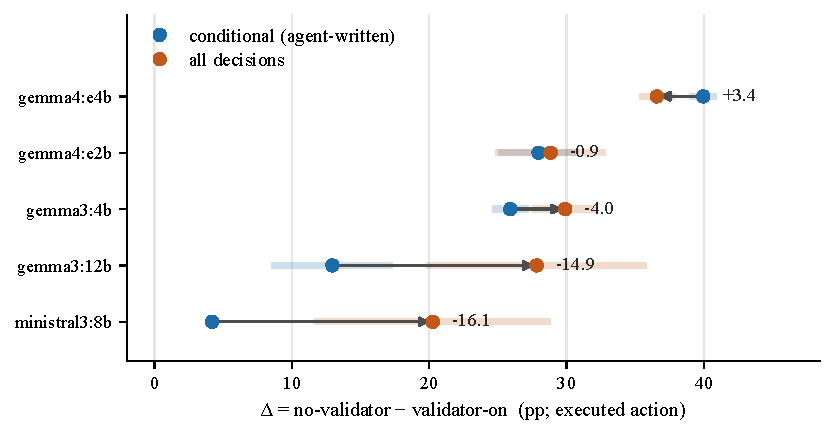
\includegraphics[width=0.98\textwidth]{../figures/active/fig3_consequence.pdf}
    \caption{\textbf{Changing the denominator changes the contrast.} Solid bars show the increase rate among high-scarcity reports; hatched bars show the rate over every decision. The y-axis is no-validator minus validator-on in percentage points. The all-decision contrast is near zero for gemma3:12b and reverses sign for ministral3:8b. These are descriptive contrasts, not causal effect estimates or corrected effect sizes.}
    \label{fig:consequence}
\end{figure*}

\section{Reporting Protocol and Limitations}
\label{sec:reporting}

The results support a small reporting protocol for governed-agent evaluations:
\begin{enumerate}[leftmargin=1.3em,itemsep=0.1em,topsep=0.2em]
    \item Report the share of decisions satisfying every agent-authored condition in both governance arms beside the conditional rate.
    \item Log the independent simulator state that corresponds to the agent report whenever such a state exists.
    \item Report an all-decision rate beside the conditional rate when the design defines one.
    \item Store the first response before a retry and the validation message that triggered the retry.
    \item When actions change the environment, preserve a trajectory or comparison run that makes the world-state dependence explicit.
\end{enumerate}

Replacing the report with a world-recorded condition is not an automatic fix. For this cell, the share with simulator-recorded shortage tier 2 or worse shifts by $+64.29\pp$. The agent-reported scarcity condition shifts by $+45.73\pp$, and the two-condition rule shifts by $+43.15\pp$. The simulator record is independent of the current response, which enables reweighting, but governance also changes that record through the reservoir loop. The alternative condition defines a different quantity, not an unaffected version of the original one.

The main limitation is missing first-attempt information. In the anchor irrigation cell, about 24.3\% of governed decisions are accepted after at least one retry. The report that preceded the accepted response is not in the frozen corpus. We therefore cannot separate a report revision within the same decision from selection into the observed accepted set.

The world-state decomposition is limited to the anchor irrigation cell, and world state is downstream of governance. The model set is small and uses models with publicly available weights; it contains no frontier models. The simulation setting and rule regime are confounded, so the claim concerns this class of coupled governance loop rather than all LLM agents.

The supplement's inventory records missing run-level recording-history fields. Finally, the Flood artifacts have source-history limitations. We do not use them to support causal claims: their cross-testbed contrast is a descriptive check, not a paired comparison or causal estimate. The B6 exclusion and unequal run counts are documented in Table~\ref{tab:cross_testbed} and the supplement.

\section{Conclusion}

Runtime governance can change the population used to evaluate an agent. In the WAGF simulations, the share of decisions with an agent-reported rule condition shifts alongside the conditional action rate. The later divergence between arms is consistent with the different world-state compositions created by the coupled environment, but this evidence does not establish a causal explanation. An all-decision rate can produce a different magnitude or direction. A conditional score should therefore be reported with its denominator, the independent world record, and the action and selection rules that produced the estimate.

\subsection*{AI Use Statement}
An AI assistant was used for language editing and for generating the non-data-bearing Figure~\ref{fig:concept}. The authors specified the figure's semantic layout, reviewed the artwork at full size and thumbnail size, and checked its labels and arrow endpoints against the manuscript. The authors independently reviewed all numerical results, study-design decisions, claims, and citations, and take responsibility for the accuracy, originality, and scientific interpretation of this submission.

\subsection*{Ethics Statement}
The study uses simulated agents and does not recruit human participants. The submission does not release local paths, private model credentials, or identifying run metadata. Any future release of source profiles or manifests will be limited to artifacts for which redistribution and anonymization have been verified.

\subsection*{Reproducibility Statement}
The main paper reports the model configurations, paired-arm design, seed-level inferential unit, action reading, and metric definitions. The supplementary package contains a frozen evidence inventory, copied machine-readable table and figure values, the cross-testbed summary source, figure regeneration commands, the generated Figure~\ref{fig:concept} staging builder, and a checklist of unavailable first-attempt fields. The quantitative evidence scripts remain in the historical WAGF evidence tree; the package records that dependency explicitly rather than claiming self-contained reruns.

No new network or GPU run is required when that frozen corpus and its scripts are available. A pre-submission manifest audit flags three historical smoke manifests as \texttt{git\_dirty=true}, so this paper does not claim bitwise reproduction of the historic runs.

\bibliographystyle{iclr2027_conference}
\bibliography{references}

\end{document}
